\documentclass[english,,man,floatsintext]{apa6}
\usepackage{lmodern}
\usepackage{amssymb,amsmath}
\usepackage{ifxetex,ifluatex}
\usepackage{fixltx2e} % provides \textsubscript
\ifnum 0\ifxetex 1\fi\ifluatex 1\fi=0 % if pdftex
  \usepackage[T1]{fontenc}
  \usepackage[utf8]{inputenc}
\else % if luatex or xelatex
  \ifxetex
    \usepackage{mathspec}
  \else
    \usepackage{fontspec}
  \fi
  \defaultfontfeatures{Ligatures=TeX,Scale=MatchLowercase}
\fi
% use upquote if available, for straight quotes in verbatim environments
\IfFileExists{upquote.sty}{\usepackage{upquote}}{}
% use microtype if available
\IfFileExists{microtype.sty}{%
\usepackage[]{microtype}
\UseMicrotypeSet[protrusion]{basicmath} % disable protrusion for tt fonts
}{}
\PassOptionsToPackage{hyphens}{url} % url is loaded by hyperref
\usepackage[unicode=true]{hyperref}
\hypersetup{
            pdftitle={Non-word repetition in Yélî Dnye},
            pdfauthor={Alejandrina Cristia~\& Marisa Casillas},
            pdfkeywords={phonology, non-word repetition, development},
            pdfborder={0 0 0},
            breaklinks=true}
\urlstyle{same}  % don't use monospace font for urls
\ifnum 0\ifxetex 1\fi\ifluatex 1\fi=0 % if pdftex
  \usepackage[shorthands=off,main=english]{babel}
\else
  \usepackage{polyglossia}
  \setmainlanguage[]{english}
\fi
\usepackage{graphicx,grffile}
\makeatletter
\def\maxwidth{\ifdim\Gin@nat@width>\linewidth\linewidth\else\Gin@nat@width\fi}
\def\maxheight{\ifdim\Gin@nat@height>\textheight\textheight\else\Gin@nat@height\fi}
\makeatother
% Scale images if necessary, so that they will not overflow the page
% margins by default, and it is still possible to overwrite the defaults
% using explicit options in \includegraphics[width, height, ...]{}
\setkeys{Gin}{width=\maxwidth,height=\maxheight,keepaspectratio}
\IfFileExists{parskip.sty}{%
\usepackage{parskip}
}{% else
\setlength{\parindent}{0pt}
\setlength{\parskip}{6pt plus 2pt minus 1pt}
}
\setlength{\emergencystretch}{3em}  % prevent overfull lines
\providecommand{\tightlist}{%
  \setlength{\itemsep}{0pt}\setlength{\parskip}{0pt}}
\setcounter{secnumdepth}{0}
% Redefines (sub)paragraphs to behave more like sections
\ifx\paragraph\undefined\else
\let\oldparagraph\paragraph
\renewcommand{\paragraph}[1]{\oldparagraph{#1}\mbox{}}
\fi
\ifx\subparagraph\undefined\else
\let\oldsubparagraph\subparagraph
\renewcommand{\subparagraph}[1]{\oldsubparagraph{#1}\mbox{}}
\fi

% set default figure placement to htbp
\makeatletter
\def\fps@figure{htbp}
\makeatother

\usepackage{fontspec}

\setmainfont{Doulos SIL} % Set main font to Doulos SIL

\title{Non-word repetition in Yélî Dnye}
\author{Alejandrina Cristia\textsuperscript{1}~\& Marisa
Casillas\textsuperscript{2}}
\date{}

\authornote{All data are made available in a repository in the
Open Science Framework. AC acknowledges the support of the Agence
Nationale de la Recherche (ANR-17-CE28-0007 LangAge, ANR-16-DATA-0004,
ANR-14-CE30-0003, ANR-17-EURE-0017); and the J. S. McDonnell Foundation
Understanding Human Cognition Scholar Award.

Correspondence concerning this article should be addressed to
Alejandrina Cristia, 29, rue d'Ulm, 75005 Paris, France. E-mail:
\href{mailto:alecristia@gmail.com}{\nolinkurl{alecristia@gmail.com}}}

\abstract{
In nonword repetition (NWR) studies, participants are presented
auditorily with an item that is phonologically legal but lexically
meaningless in the local language. NWR scores are thought to reflect
long-term phonological knowledge as well as online phonological working
memory and flexible production patterns. In this study, we report on NWR
results among children learning Yélî Dnye, an isolate spoken on Rossel
Island in Papua New Guinea, with an unusually dense phonological
inventory. This study contributes to three lines of research. First, we
document that non-word items containing typologically rare sounds are
repeated without changes less often that non-words containing more
common sounds. Second, we document rather weak effects of item length,
contributing to other research suggesting that length effects may be
language-specific. Third, we do not find strong individual variation
effects in this population, contrary to previous results documenting
strong age-related effects. Together, these data provide a unique view
of online phonological processing in a seldom-studied language, and
contribute to both typological and language acquisition research.


}

\begin{document}
\maketitle

\subsection{TODO Alex}\label{todo-alex}

\begin{itemize}
\tightlist
\item
  check again if all fields are explained
\item
  set up OSF (or revise if already there)
\item
  implement decisions on prop phones \& patterns nwr mp
\item
  revise bullet points for discussion
\end{itemize}

\subsection{TODO Middy}\label{todo-middy}

\begin{itemize}
\tightlist
\item
  double check my frequency entries in segments.xlsx using the search
  function in \url{https://phoible.org/parameters}; take a look at
  \url{http://phoible.github.io/conventions/} in case you see something
  about double articulation (I didn't find tp or lBj) 
\item
  draft discussion
\end{itemize}

\subsection{Introduction}\label{introduction}

Children's perception and production of phonetic and phonological units
continues developing well beyond the first year of life, even extending
into middle childhood (e.g., Hazan \& Barrett, 2000). Much of the
evidence for later phonological development comes through the use of
nonword repetition (NWR) tasks. In a NWR task, participants hear a short
word-like form that is phonologically legal but lexically meaningless in
the language(s) they are learning. After hearing this non-word, the
participant's task is to try to immediately and precisely repeat it. NWR
scores are thought to reflect long-term phonological knowledge (to
perceive the item precisely despite not having heard it before) as well
as online phonological working memory (to encode the item in the
interval between hearing it and saying it back) and flexible production
patterns (to produce the item precisely despite not having pronounced it
before).

NWR has been used to seek answers to a variety of theoretical questions,
including what the links are between phonology, working memory, and the
lexicon (Bowey, 2001), and how extensively apparent phonological
constraints found in the lexicon affect online production (Gallagher,
2014). NWR is also frequently used in applied contexts, notably as a
diagnostic tool for language delays and disorders (Estes, Evans, \&
Else-Quest, 2007). Since non-words can be generated in any language, it
has attracted the attention of researchers working in multilingual and
linguistically diverse environments, particularly in Europe (Action,
2009; Meir, Walters, \& Armon-Lotem, 2016). However, it has seldom been
used outside of Europe and North America (with exceptions including
Gallagher, 2014, and Cristia, Farabolini, Scaff, Havron, and Stieglitz
(2020)). Further, the languages it has been used with have historically
had small to moderate phonological inventories (Maddieson, 2005).

In the present study, we use NWR to investigate the phonological
development of children learning Yélî Dnye, an isolate language spoken
in Papua New Guinea (PNG) that has a large and unusually dense
phonological inventory. The study was designed to contribute to multiple
aspects of our understanding of phonological development: First, we
included a subset of non-word items with typologically rare and/or
challenging sounds to ask whether these rare sounds are disadvantaged in
perception and/or production, both in terms of overall repetition scores
and patterns of mispronunciation. Second, we varied the length (in
syllables) of non-words to investigate the impact of word length on
repetition and mispronunciation; previous NWR research has shown
variable effects of length between populations. Third, these data give a
first impression of how this task is responded to in a rarely-studied
language and culture; we add to this by further investigating whether
there are structured sources that account for individual variation in
our sample.

Before jumping into the details of our study design we first give an
overview of Yélî Dnye phonology as well as a brief ethnographic review
of the developmental environment on Rossel Island. Since NWR has been
almost exclusively used in urban, industrialized populations (see
Cristia et al., 2020 for an exception), we provide this additional
ethographic information to contextualize the adaptations we have made in
running the task and in gathering age and other demographic information,
compared to what is typical in urban, industrialized settings.

\subsubsection{Yélî Dnye phonology}\label{yuxe9luxee-dnye-phonology}

Yélî Dnye is an isolate language (presumed Papuan) spoken by
approximately 7,000 people residing on Rossel Island, an island found at
the far end of the Louisiade Archipelago in Milne Bay Province, Papua
New Guinea. The Yélî sound system, much like its baroque grammatical
system (Levinson, accepted), is unlike any other in the region.

With only four primary places of articulation (bilabial, alveolar,
post-alveolar, and velar) and no voicing contrasts, the phonological
inventory is remarkably packed with acoustically similar segments. The
core oral stop set includes both singleton (/p/, /t/, /ṭ/, and /k/) and
doubly-articulated (/tp/, /ṭp/, /kp/) segments, with full nasal
equivalents (/m/, /n/, /ṇ/, /ŋ/, /nm/, /ṇm/, /ŋm/), and with a
substantial portion of them contrastively pre-nasalized or nasally
released (/mp/, /nt/, /ṇṭ/, /ŋk/, /nmtp/, /ṇmṭp/, /ŋmkp/, /ṭṇ/, /kŋ/,
/ṭpṇm/, /kpŋm/). A large number of this combinatorial set can further be
contrastively labialized, palatalized on release, or both (e.g., /pʲ/,
/pʷ/, /pʲʷ/; /tpʲ/; /ṇmḍbʲ/; see Levinson (accepted) for
details).\footnote{We use Levinson's (accepted) under-dot notation
  (e.g., /ṭ/) to indicate the post-alveolar place of articulation; these
  stops are, articulatorily, somewhat variable in place, with at least
  some tokens produced fully sub-apically. In approximating
  cross-linguistic segment frequency below we use the corresponding
  retroflex for each stop segment (e.g., /ʈ/, /ʈp/, /ɳ/).} The
consonantal inventory also includes a number of non-nasal continuants
(/w/, /j/, /ɣ/, /l/, /βʲ/, /lʲ/, /lβʲ/). Vowels in Yélî Dnye may be oral
or nasal, short or long. The 10 oral vowel qualities, which span four
levels of vowel height, (/i/, /ɯ/, /u/, /e/, /o/, /ə/, /ɛ/, /ɔ/, /æ/,
/ɑ/) can be produced as short and long vowels, with 7 of these able to
appear as short and long nasal vowels as well /ĩ/, /ũ/, /ə̃/, /ɛ̃/, /ɔ̃/,
/æ̃/, /ɑ̃/).

In total, Yélî Dnye uses 90 distinctive segments (not including an
additional 3 rarely used consonants), far outstripping the phonemic
inventory size of other documented Papuan languages (Foley, 1986;
Levinson, accepted) and includes at least two contrasts not yet been
documented elsewhere (labial-coronal double-articulations with dental
vs.~post-alveolar coronal placement for both oral and nasal stops,
Ladefoged \& Maddieson, 1996; Maddieson \& Levinson, in preparation).

Most words in Yélî Dnye are bisyllabic (\textasciitilde{}50\%), with
monosyllabic words (\textasciitilde{}40\%) appearing most commonly after
that, and with tri-and-above syllabic words appearing least frequently
(\textasciitilde{}10\%; based on \textgreater{}5800 lexemes in the most
recent Yélî Dnye dictionary at time of writing, Levinson, accepted). The
vast majority of syllables use a CV format. A small portion of the
lexicon features words with a final closed syllable, limited to codas of
-/m/, -/p/, or -/j/ (e.g., `ndap' (Spondylus shell) /ṇṭæp/). However, in
spontaneous speech an epenthetic /ɯ/ is often inserted after word-final
coda, yielding a CVCV structure instead (e.g., `ndapî' /`ṇṭæ.pɯ/). This
process is used frequently with English loan words that have a coda
(e.g., 'ponî' (phone) /`pɔ.nɯ/). An even smaller portion of the lexicon
features words starting with a vowel (e.g., 'ala' (here) /æ.'læ/), but
these are limited to /æ/-. Finally, the lexicon features a handful of
single-vowel grammatical morphemes (see Levinson (accepted) for
details).

\subsubsection{The Yélî community}\label{the-yuxe9luxee-community}

Most speakers of Yélî Dnye grow up speaking it monolingually until they
begin attending school around the age of 7; school instruction is in
English. While monolingual Yélî Dnye upbringing is common, multilingual
families are not unusual, particularly in the region around the Catholic
Mission---the same region in which the current data were
collected---where there is a higher incidence of married-in mothers from
other islands (Brown \& Casillas, in press). Children in these
multilingual families grow up speaking Yélî Dnye plus English, Tok
Pisin, and/or another language(s) from the region.

Most Yélî people are swidden horticulturalists, raising a variety of
tubers (e.g., yams, manioc, taro), coconut, banana, and more in their
gardens. In addition to garden foods, Yélî children grow up eating fish
and foraging for shellfish and nuts, which provide a regular source of
extra protein. The typical household in our dataset includes seven
individuals and is situated among a collection of 4 or more other
households, with structures often arranged around an open grassy area.
These household clusters are organized by patrilocal relation, such that
they typically comprise a set of brothers, their wives and children, and
their mother and father, with neighboring hamlets also typically related
through the patriline.

Laying 250 nautical miles off the coast of mainland PNG and surrounded
by a barrier reef, transport to and from the island is both infrequent
and irregular. There is no electricity system (we use solar panels) or
motor vehicles on the island, save dinghys with outboard motors that,
even when there is deisel available, are primarily reserved for medical
transport. There is a medical radio connection at the health clinic,
located at the Catholic Mission, via which news and messages are often
passed to and from mainland PNG. There is also a cellular tower on the
island, though it is often inoperative, usually for multiple months or
years at a time. As such, access to news and outside connections,
including international phone calls and digital exchanges that require
significant data transfer, is typically unavailable. Our data collection
is therefore limited to the duration of the researchers' on-island
visits.

Despite restricted outside contact, formal education is a priority for
many Yélî families. A recent study surveying more than 40 parents of
young children in this region of the island found that nearly all
parents completed 6 or more years of education, with 65\% of mothers and
49\% of fathers completing the full range of locally available education
(\textasciitilde{}9 years), with around half of those parents having
pursued an additional 2+ years of education on other islands in the
region or on mainland PNG (Casillas, Brown, \& Levinson, 2020). While
there are a handful of local schools around the island, these may be
well out of walking distance for many children (i.e., more than 1 hour
on foot or by canoe each day). It is very common for households situated
close to schools to billet their school-aged relatives during the
weekdays (sometimes the weekends too, if the child's home is very far)
for long segements of each school year. Combined with practices of
collective child guardianship within each close-knit hamlet, the
practical consequence of this billeting for researchers is that adult
consent can often come from a combination of aunts, uncles, adult
cousins, and grandparents standing in for the child's biological
parents. On top of this, child assent is culturally pertinent, as child
independence is encouraged and respected from toddlerhood onward (Brown
\& Casillas, in press).\footnote{For these reasons, we were unable to
  record precise details for a few children, including child date of
  birth, parent age in years, and parent education.} Finally, as
mentioned, the language of schooling in this region is English, and so
the majority of teens and adults on the island speak some English---many
speak it very fluently.

While work on Yélî language development is growing (e.g., Brown, 2011,
2014; Brown \& Casillas, in press; Casillas et al., 2020; Liszkowski,
Brown, Callaghan, Takada, \& de Vos, 2012), our knowledge of children's
linguistic development is quite limited, and research into their
phonological development in particular has only just begun (e.g., Peute,
Fikkert, \& Casillas, In preparation). What we do know about the early
language environment is that, while direct speech to children under 3;0
is relatively infrequent throughout the day (Casillas et al., 2020),
shared caregiving practices and a near-universal fondness for social
interaction with young children ensure that speech directed to children
comes from all types of speakers: women, men, and other children (Bunce
et al., under review; Casillas et al., 2020). While speech from women
predominates in young children's speech environments on Rossel, as it
does elsewhere (Bergelson et al., 2019; Bunce et al., under review),
there is a significant and marked increase in child-directed speech from
other children as infants get older (Bunce et al., under review;
Casillas et al., 2020). This increase in child-directed speech from
other children is attributed to the fact that, starting around age 2,
children often spend large swaths of the day playing, swimming, and
foraging for fruit, nuts, and shellfish in large (\textasciitilde{}10
members) independent and mixed-age child play groups (Brown \& Casillas,
in press; Casillas et al., 2020).

\subsubsection{NWR design and analysis
adaptations}\label{nwr-design-and-analysis-adaptations}

In a basic NWR task, the participant listens to a production of a
word-like form, such as /bilik/, and then repeats back what they heard
without changing any phonological feature that is contrastive in the
language. For instance, in English, a response of {[}bilig{]} or
{[}pilik{]} would be scored as incorrect; a response {[}biilik{]}, where
the vowel is lengthened without change of quality would be scored as
correct, because English does not have a general feature of contrastive
vowel length. There is some variation in how past NWR studies have
designed the presentation procedure and structure of items. For example,
while items are often presented orally by the experimenter (Torrington
Eaton, Newman, Ratner, \& Rowe, 2015), an increasing number of studies
have turned instead to playing back pre-recorded stimuli in order to
increase control in stimulus presentation (Brandeker \& Thordardottir,
2015). Additionally, while some studies have used 10-15 non-words,
others have employed up to 46 unique items (Piazzalunga, Previtali,
Pozzoli, Scarponi, \& Schindler, 2019). Authors also often modulate
structural complexity, typically measured in terms of item length
(measured in number of syllables) and/or syllable structure (open as
opposed to closed syllables, Gallon, Harris, \& Van der Lely, 2007).

Previous work typically steers clear of articulartorily and/or
acoustically challenging sounds, but we included some in our experiment
to more adequately represent Yélî Dnye's phonology. We ultimately used a
relatively large number of items that would enable us to explor both
variation in structural complexity and in more vs.~less challenging
sounds. However, aware that this large item inventory might render the
task longer and more tiresome, we split items across children (see
below). Naturally, designing the task in this way may render the study
of individual variation within the population more difficult because
different children are exposed to different items. However, a review of
previous work on individual variation suggested to us that effects of
individual differences in NWR are relatively small, and would not be
detectable with the sample size that we could collect during our short
visit. That said, we contribute to the literature by also reporting
descriptive analyses of individual variation that could potentially be
integrated in meta-analytic efforts.

Based on previous work, we looked at potential changes with age (Farmani
et al., 2018; Kalnak, Peyrard-Janvid, Forssberg, \& Sahlén, 2014; Vance,
Stackhouse, \& Wells, 2005), and differences relating to bilingual
language exposure (Brandeker \& Thordardottir, 2015; Meir \&
Armon-Lotem, 2017; Meir et al., 2016). Previous work typically finds no
significant differences as a function of maternal education (e.g.,
Farmani et al., 2018; Kalnak et al., 2014; Meir \& Armon-Lotem, 2017) or
child gender (Chiat \& Roy, 2007). Although past research has not often
investigated potential effects of birth order on NWR, there is a sizable
literature on these effects in other language tasks (Havron et al.,
2019), and therefore we report on these too.

\subsubsection{Research questions}\label{research-questions}

After some preliminary analyses to set the stage, we address the
following questions:

\begin{itemize}
\tightlist
\item
  Does the cross-linguistic frequency of sounds predict NWR scores? Are
  rarer sounds more often substituted by commoner sounds?
\item
  How does score change as a function of item length in number of
  syllables?
\item
  Is individual variation attributable to child age, sex, birth order,
  monolingual status, and/or parental education?
\end{itemize}

In view of the hypothesis-driven nature of this work, we had considered
boosting the interpretational value of this evidence by announcing our
analysis plans prior to conducting them. However, we realized that even
pre-registering an analysis would be equivocal because we would not have
enough power to look at all relationships of interest, in many cases
possibly not enough to detect any of the known effects, given their
variability across studies. To illustrate this issue, we portray in
Figure 1 studies in which children's NWR scores were gathered between 4
and 12 years of age, and reported separately for items that are
relatively short (1-2 syllables) versus longer items (3-4 syllables).
Notice that the effect of stimulus length is minuscule among Italian
children (Piazzalunga et al., 2019), but considerable among Tsimane'
children (Cristia et al., 2020), where a drop of 40 percentage points is
observed at all ages. A similar large difference in NWR scores for short
versus long items was observed among Arabic children (Jaber-Awida,
2018). Even the effect of age is unstable in this sample of studies.
Whereas it is quite clear that children's NWR scores increase in the
Italian data, age effects are less stable among Tsimane' children.
Therefore, all analyses in the present study are descriptive and should
be considered exploratory.

\begin{figure}
\centering
\includegraphics{manuscript_files/figure-latex/prevlit-fig-1.pdf}
\caption{\label{fig:prevlit-fig}NWR scores as a function of age (in years)
and item length for comparable studies. Arabic data from Jaber et al.
(2018); Italian data from Piazzalunga et al. (2019); Tsimane' from
Cristia et al. (2020); Yélî data from the present study.}
\end{figure}

\subsection{Methods}\label{methods}

\subsubsection{Stimuli}\label{stimuli}

Many NWR studies are based on a fixed list of 12-16 items that vary in
length between 1 and 4 syllables, often additionally varying syllable
complexity and/or cluster presence and complexity, and always meeting
the condition that they do not mean anything in the target language
(e.g., Balladares, Marshall, \& Griffiths, 2016; Wilsenach, 2013). We
kept the same variation in item length and requirement for not being
meaningful in the language, but we did not vary syllable complexity or
clusters because these are vanishingly rare in Yélî Dnye. We also
increased the number of items an individual child would be tested on,
such that a child would get up to 23 items to repeat (other work has
also used up to 24-30 items: Jaber-Awida, 2018; Kalnak et al., 2014),
with the entire test inventory of 44 items distributed across children.

A first list of candidate items was generated during a trip to the
island in 2018 by selecting simple consonants (/p/, /t/, /ṭ/, /k/, /m/,
/n/, /w/, /y/) and vowels (/i/, /o/, /u/, /a/, /e/) and combining them
into consonant-vowel syllables, then sampling the space of 1- to
4-syllable sequences. These candidates were automatically removed from
consideration if they appeared in Levinson's (2015) dictionary. The
second author presented them orally to three local research assistants,
all native speakers of Yélî Dnye, who were repeated each form, as they
would in an NWR task, and additinally let the experimenter know if the
item was in fact a word or phrase in Yélî Dnye. Any item reported to
have a meaning or a strong association with another word form or meaning
was excluded.

A second list of candidate items was generated in 2019 by selecting
complex consonants and systematically crossing them with all the vowels
in the Yélî Dnye inventory to produce consonant-vowel monosyllabic
forms. As before, items were automatically excluded if they appeared in
the dictionary. Additionally, since perceiving vowel length in isolated
monosyllables is challenging, any item that had a short/long lexical
neighbor was excluded. Because there is still much to discover about the
phonology and phonetics of Yélî Dnye (Levinson, accepted), it was also
possible that we initially generated items with illegal, but currently
undocumented constraints. Therefore, we made sure that the precise
consonant-vowel sequence occurred in some real word in the dictionary
(i.e., that there was a longer word included the monosyllable as a
subsequence). These candidates were then presented to one informant, for
a final check that they did not mean anything. Together with the 2018
selection, they were recorded, based on their orthographic forms, using
a Shure SM10A XLR dynamic headband microphone and an Olympus WS-832
stereo audio recorder (using an XLR to mini-jack adapter) by the same
informant, monitored by the second author for clear production of the
phonological target. The complete recorded list was finally presented to
two more informants, who were able to repeat all the items and who
confirmed there were no real words present. Despite these checks, one
monosyllable was ultimately frequently identified as a real word in the
resulting data (intended ``yî'' /yɯ/; identified as ``yi'' /yi/,
\emph{tree}). This item is removed from the analyses below.

The final list includes: three practice items; 20 monoysllables
containing sounds that are less frequent in the world's languages than
singleton plosives; 8 bisyllables; 12 trisyllables; and 4
quadrisyllables (see Table 2).

\begin{table}

\caption{\label{tab:tab2-stims}NWR stimuli in orthographic and phonological representations.}
\centering
\begin{tabular}[t]{llllllllll}
\toprule
\multicolumn{2}{c}{Practice} & \multicolumn{2}{c}{Monosyll} & \multicolumn{2}{c}{Bisyll} & \multicolumn{2}{c}{Trisyll} & \multicolumn{2}{c}{Tetrasyll} \\
\cmidrule(l{3pt}r{3pt}){1-2} \cmidrule(l{3pt}r{3pt}){3-4} \cmidrule(l{3pt}r{3pt}){5-6} \cmidrule(l{3pt}r{3pt}){7-8} \cmidrule(l{3pt}r{3pt}){9-10}
Orth. & Phon. & Orth. & Phon. & Orth. & Phon. & Orth. & Phon. & Orth. & Phon.\\
\midrule
nopimade & nɔpimæṭɛ & dp:a & ṭp̃æ & kamo & kæmɔ & dimope & ṭimɔpɛ & dipońate & ṭipɔnætɛ\\
poni & pɔni & dpa & ṭpæ & kańi & kæni & diyeto & ṭijɛtɔ & ńomiwake & nɔmiwækɛ\\
wî & wɯ & dpâ & ṭpɑ & kipo & kipɔ & meyadi & mɛjæṭi & todiwuma & tɔṭiwumæ\\
 &  & dpê & ṭpə & ńoki & nɔki & mituye & mitujɛ & wadikeńo & wæṭikɛnɔ\\
 &  & dpéé & ṭpeː & ńomi & nɔmi & ńademo & næṭɛmɔ &  & \\
\addlinespace
 &  & dpi & ṭpi & piwa & piwæ & ńayeki & næjɛki &  & \\
 &  & dpu & ṭpu & towi & tɔwi & ńuyedi & nujɛṭi &  & \\
 &  & gh:ââ & ɣ̃ɑː & tupa & tupæ & pedumi & pɛṭumi &  & \\
 &  & ghuu & ɣuː &  &  & tiwuńe & tiwunɛ &  & \\
 &  & kp:ââ & kp̃ɑː &  &  & tumowe & tumɔwɛ &  & \\
\addlinespace
 &  & kpu & kpu &  &  & widońe & wiṭɔnɛ &  & \\
 &  & lv:ê & lβʲ̃ə &  &  & wumipo & wumipɔ &  & \\
 &  & lva & lβʲæ &  &  &  &  &  & \\
 &  & lvi & lβʲi &  &  &  &  &  & \\
 &  & t:êê & t̃əː &  &  &  &  &  & \\
\addlinespace
 &  & tp:a & tp̃æ &  &  &  &  &  & \\
 &  & tpâ & tpɑ &  &  &  &  &  & \\
 &  & tpê & tpə &  &  &  &  &  & \\
\bottomrule
\end{tabular}
\end{table}

A Praat script (Boersma \& Weenink, 2020) was written to randomize this
list 20 times, and split it into two sublists, to generate 40 different
elicitation sets. The 40 elicitation sets are available online from
\url{https://osf.io/5qspb}. The split had the following constraints:

\begin{itemize}
\tightlist
\item
  The same three items were selected as practice items and used in all
  40 elicitation sets
\item
  Splits were done within each length group from the 2018 items (i.e.,
  separately for 2-, 3-, and 4-syllable items); and among onset groups
  for the difficult monosyllables generated in 2019 (i.e., all the
  monosyllables starting with /tp/ were split into 2 sublists). Since
  some of these groups had an odd number of items, one of the sublists
  was slightly longer than the other (20 vs.~23).
\item
  Once the sublist split had been done, items were randomized such that
  all children heard first the 3 practice items in a fixed order (1-,
  2-, and 4-syllable), a randomized version of their sublist selection
  of difficult onset items, and randomized versions of their 2-syllable,
  then 3-syllable, and finally 4-syllable items.
\end{itemize}

\subsubsection{Procedure}\label{procedure}

In adapting the typical NWR procedure for this context, we balanced
three desiderata: That children would not be unduly exposed to the items
before they themselves had to repeat them (i.e., from other children who
had participated); that children would feel comfortable doing this task
with us; and that community members would feel comfortable having their
children do this task with us.

We ran children in batches, testing within a handful of hamlet clusters
spread across the northeastern region of the island. Because space
availability was limited in different ways from hamlet to hamlet, the
places where elicitation happened varied across testing sites. We tested
in four different sites, only making a single visit to each, conducting
back-to-back testing of all eligible children present at the time of our
visit in order to prevent the items `spreading' between children through
hearsay. In the first hamlet, we tested children in five different
places, with some children being tested inside a house and others tested
on the veranda. The complete list of places and the ways in which they
met the desiderata mentioned above can be found in the raw data,
available from online supplementary materials. Whenever children living
in the same household were tested, we tried to test children in age
order, from oldest to youngest, to minimize intimidation for younger
household members, and always using different elicitaiton sets.

We fitted the child with a headset microphone (Shure SM10A or WH20 XLR
with a dynamic microphone on a headband, most children using the former)
that fed into the left channel of a Tascam DR40x digital audio recorder.
The headsets were designed for adult use and could not be comfortably
seated on many children's heads without a more involved adjustment
period. To minimize adjustment time, which was uncomfortable for some
children given the proximity of the experimenter and equipment, we
placed the headband on children's shoulders in these cases, carefully
adjusting the microphone's placement so that it was still close to the
child's mouth. A research assistant who spoke Yélî Dnye natively sat
next to the child throughout the task to provide instructions and, if
needed, encouragement. The research assistant coached the child
throughout to task to make sure that they understood what they were
expected to do. An experimenter (the first author) delivered the
pre-recorded stimuli to the research assistant and the child over
headphones.

The first phase of the experiment involved making sure the child
understood the task. We explained the task orally presented the first
practice item. At this point, many children did not say anything in
response, at which point we initiated the following procedure: First,
the assistant insisted the child make a response. If the child still did
not say anything, the assistant said a real word and then asked the
child to repeat it, then another and another. If the child could repeat
real words correctly, we provided the first training item over
headphones again for children to repeat. Most children successfully
started repeating the items at this point, but a few needed further
help. In this case, the assistant modeled the behavior (i.e., the child
and assistant would hear the item again, and the assistant would repeat
it; then we would play the item again and ask the child to repeate it).
A small minority of children still failed to repeat the item at this
point. If so, we tried again with the second training item, at which
point some children got it and could continue. A fraction of the
remaining children, however, failed to repeat this second training item,
as well as the third one, in which case we stopped testing altogether
(see Participants section for exclusions).

The second phase of the experiment involved running the child through
the list of test items randomly assigned to them. This was done in the
same manner as the practice items: the stimulus was played over the
headphones, and then the child repeated it aloud. NWR studies vary in
whether children are allowed to hear and/or repeat the item more than
one time. We had a fixed procedure for the test items (i.e., the
non-practice items) in which the child was alowed to make a further
attempts if their first attempt was judged erroneous in some way by the
assistant. The procedure worked as follows: When the child made an
attempted a repeat, the assistant indicated to the experimenter whether
the child's production was correct or not. If correct, the experimenter
would whisper this note of correct repetition into a separate headset
that fed into the right channel of the same Tascam and the group moved
on to the next item. If not, the child was allowed to try again, with up
to five attempts allowed before moving on to the next item. Children
were not asked to make repetitions if they did not produce a first
attempt.

In total, test sessions took approximately XX minutes on average, with
XX of those minutes attributed to practice and XX to the actual test
list.

\subsubsection{Coding}\label{coding}

The first author then annotated the onset and offset of all children's
productions from the audio recording using Praat audio annotation
software (Boersma \& Weenink, 2020), then wrote and ran a script to
extract these tokens, pairing them with their original auditory target
stimulus, and writing these audio pairs out to short .wav files. The
assistant then listened through all these productions, one target item
at a time, with productions for each target item presented in a random
order across children and repetitions. The assistant indicated in a
notebook whether each production was a correct or incorrect repetition
and orthographically transcribed the production, noting when the child
uttered a recognizable word or phrase and adding the translation
equivalent of that word/phrase into English. The assistant also provided
some general examples of the types of errors children made without
making specific reference to Yélî sounds or the items in the elicitation
sets.

\subsubsection{Analyses}\label{analyses}

In addition to a binary word-level exact repetition score we scored
items in terms of the number of phonemes that could be aligned across
the target and attempt, divided by the number of phonemes of whichever
item was longer (the target or the attempt; see also Cristia et al.,
2020). Although previous work does not use distance metrics, we
additionally report these. For instance, recall our example of an
English target being /bilik/ with an imagined response {[}bilig{]}. We
would score this response as follows: at the whole item level this
production would receive a score of zero (because the repetition is not
exact); at the phoneme level this production would receive a score of
80\% (4 out of 5 phonemes repeated exactly); and the phone-based
Levenshtein distance for this production is 20\% (because 20\% of
phonemes were substituted or deleted).\\

Additionally, we estimated the typological frequency of all phonological
segments used in the target items using the PHOIBLE cross-linguistic
phonological inventory database (Moran \& McCloy, 2019). For each phone
in our task, we extracted the number and percentage of languages noted
to have that phone in its inventory. While PHOIBLE is an unprecedentedly
comprehensive database, with phonological inventory data for over 2000
languages at the time these data were analyzed, it is of course still
far from complete, so estimated frequencies should be taken with a pinch
of salt. In both PHOIBLE and UPSID---another large phonemic inventory
database---note that nearly half of the segment types only appear in a
single language (Steven Moran, personal communication; see also
\href{http://web.phonetik.uni-frankfurt.de/upsid_info.html}{web.phonetik.uni-frankfurt.de/upsid\_info.html}).
It is therefore unsurprising that we did not find three of our segments
(/lβʲ/, /ṭp/, and /tp/) in the database. Following the general pattern
that many phones only appear once cross-linguistically, even in large
databases, we treat our ``missing'' phones as having a frequency of 1,
with a (rounded) percentage of 0\%.

Finally, when describing children's patterns of errors, we take all
repetitions of a given target into account. We describe the proportion
of items where the change resulted in a real word (semantic errors); as
well as deletions, additions, and substitutions.

\subsubsection{Participants}\label{participants}

This study was approved as part of a larger research effort by the
second author. The line of research was evaluated by the Radboud
University Faculty of Social Sciences Ethics Committee (Ethiek Commissie
van de faculteit der Sociale Wetenschappen; ECSW) in Nijmegen, The
Netherlands (original request: ECSW2017-3001-474 Manko-Rowland;
amendment: ECSW-2018-041). Participation was voluntary; children were
invited to participate following indication of approval from an adult
caregiver. Regardless of whether they completed the task, children were
given a small snack as compensation. Children who showed initial
interest but then decided not to participate were also given the snack.

We tested a total of 55 children from 38 families spread across four
hamlets. We excluded test sessions from analysis for the following
reasons: refused participation or failed to repeat items presented over
headphones even after coaching (N=8), spoke too softly to allow offline
coding (N=5), or were 13 years old or older (N=2; we tested these
teenagers to put younger children at ease). The remaining 40 children
(14 girls) were aged 6.98 years (range 3.92-11.03 years). Among these
children were 34 only exposed to Yélî Dnye at home and 6 children
exposed to one or more other languages at home. Maternal years of
education averaged 8.22 years (range 6-12 years).\footnote{Years of
  education is difficult to precisely pinpoint in this context.
  Schooling beyond grade 8 takes place off-island and enrollment is tied
  to an ability to pay that year's school fees, seasonal interruptions
  to school opening times, familial obligations, and more. We asked
  parents to report their highest completed level of education. We then
  record the number of years entailed by having completed that level
  under ideal conditions. This method results in many esimates around
  typical ``graduation'' times (e.g., graduating from primary education
  before starting secondary education).} In terms of birth order, 6 were
first borns, 5 second, 2 third, 7 forth, 5 fifth, and 1 sixth.

\subsection{Results}\label{results}

\subsubsection{Preliminary analyses}\label{preliminary-analyses}

\begin{figure}
\centering
\includegraphics{manuscript_files/figure-latex/Fig1-first-vs-others-1.pdf}
\caption{\label{fig:Fig1-first-vs-others}Whole-item NWR scores for
individual participants averaging separately their first attempts and
all other attempts.}
\end{figure}

We first checked whether whole-item NWR scores varied between first and
subsequent presentations of an item by averaging word-level scores at
the participant level separately for first attempts and subsequent
repetitions. We excluded 1 children who did not have data for one of
these two types. As shown in Figure \ref{fig:Fig1-first-vs-others},
participants' mean word-level scores became more heterogeneous in
subsequent repetitions. Surprisingly, whole-item NWR scores for
subsequent repetitions (M = 40, SD = 26) were on average lower than
first ones (M = 64, SD = 15), t(38) = 6.28, p = 0; Cohen's d = 1.14).
Given uncertainty in whether previous work used first or all
repetitions, and given that score here declined and became more
heterogeneous in subsequent repetitions, we focus the remainder of our
analyses only on first repetitions.

Taking into account only the first attempts, we averaged attempts by
each of the 40 children who had data for first attempts; their ages
ranged from 3 to 10 (M = 6.50, SD = 1.50).

The overall NWR score was M = 64\% (SD = 15\%), Cohen's d = 4.36. Scores
based on phonemes are even higher M = 78\% (SD = 9\%), Cohen's d = 8.55.
The phoneme-based normalized Levenshtein distance was M = 22\% (SD =
9\%), meaning that about a fifth of phonemes were were substituted,
inserted, or deleted (the normalized Levenshtein distance is the
complement of phoneme-based scores).

\subsubsection{NWR as a function of cross-linguistic phone
frequency}\label{nwr-as-a-function-of-cross-linguistic-phone-frequency}

In this analysis, we were interested in variation in whole-item NWR
scores as a function of the average frequency with which sounds
composing individual target words are found in languages over the world.
To look at this, we fit a mixed logistic regression, in which the
outcome variable was whether the non-word was correctly repeated or not.
The fixed effects of interest was the average cross-linguistic phone
frequency; we also included child age as a control fixed effect, and
child ID \& target ID as random variables.

We could include 850 observations, from 40 children producing in any
given trial one of 41 potential target words. The analysis revealed a
main effect of age (ß = 0.33, SE ß = 0.13, p = 0.01); and a significant
estimate for the scaled average cross-linguistic frequency of phones in
the target words (ß = 0.82, SE ß = 0.18, p = 0): Target words with
phones found more frequently across languages had a higher proportion of
words that were correctly repeated, as clear in Figure 2. Averaging
across items and participants, the Pearson correlation between scaled
average cross-linguistic phone frequency and whole-item NWR scores was r
r(31) = 0.63.

\begin{figure}[!t]

{\centering 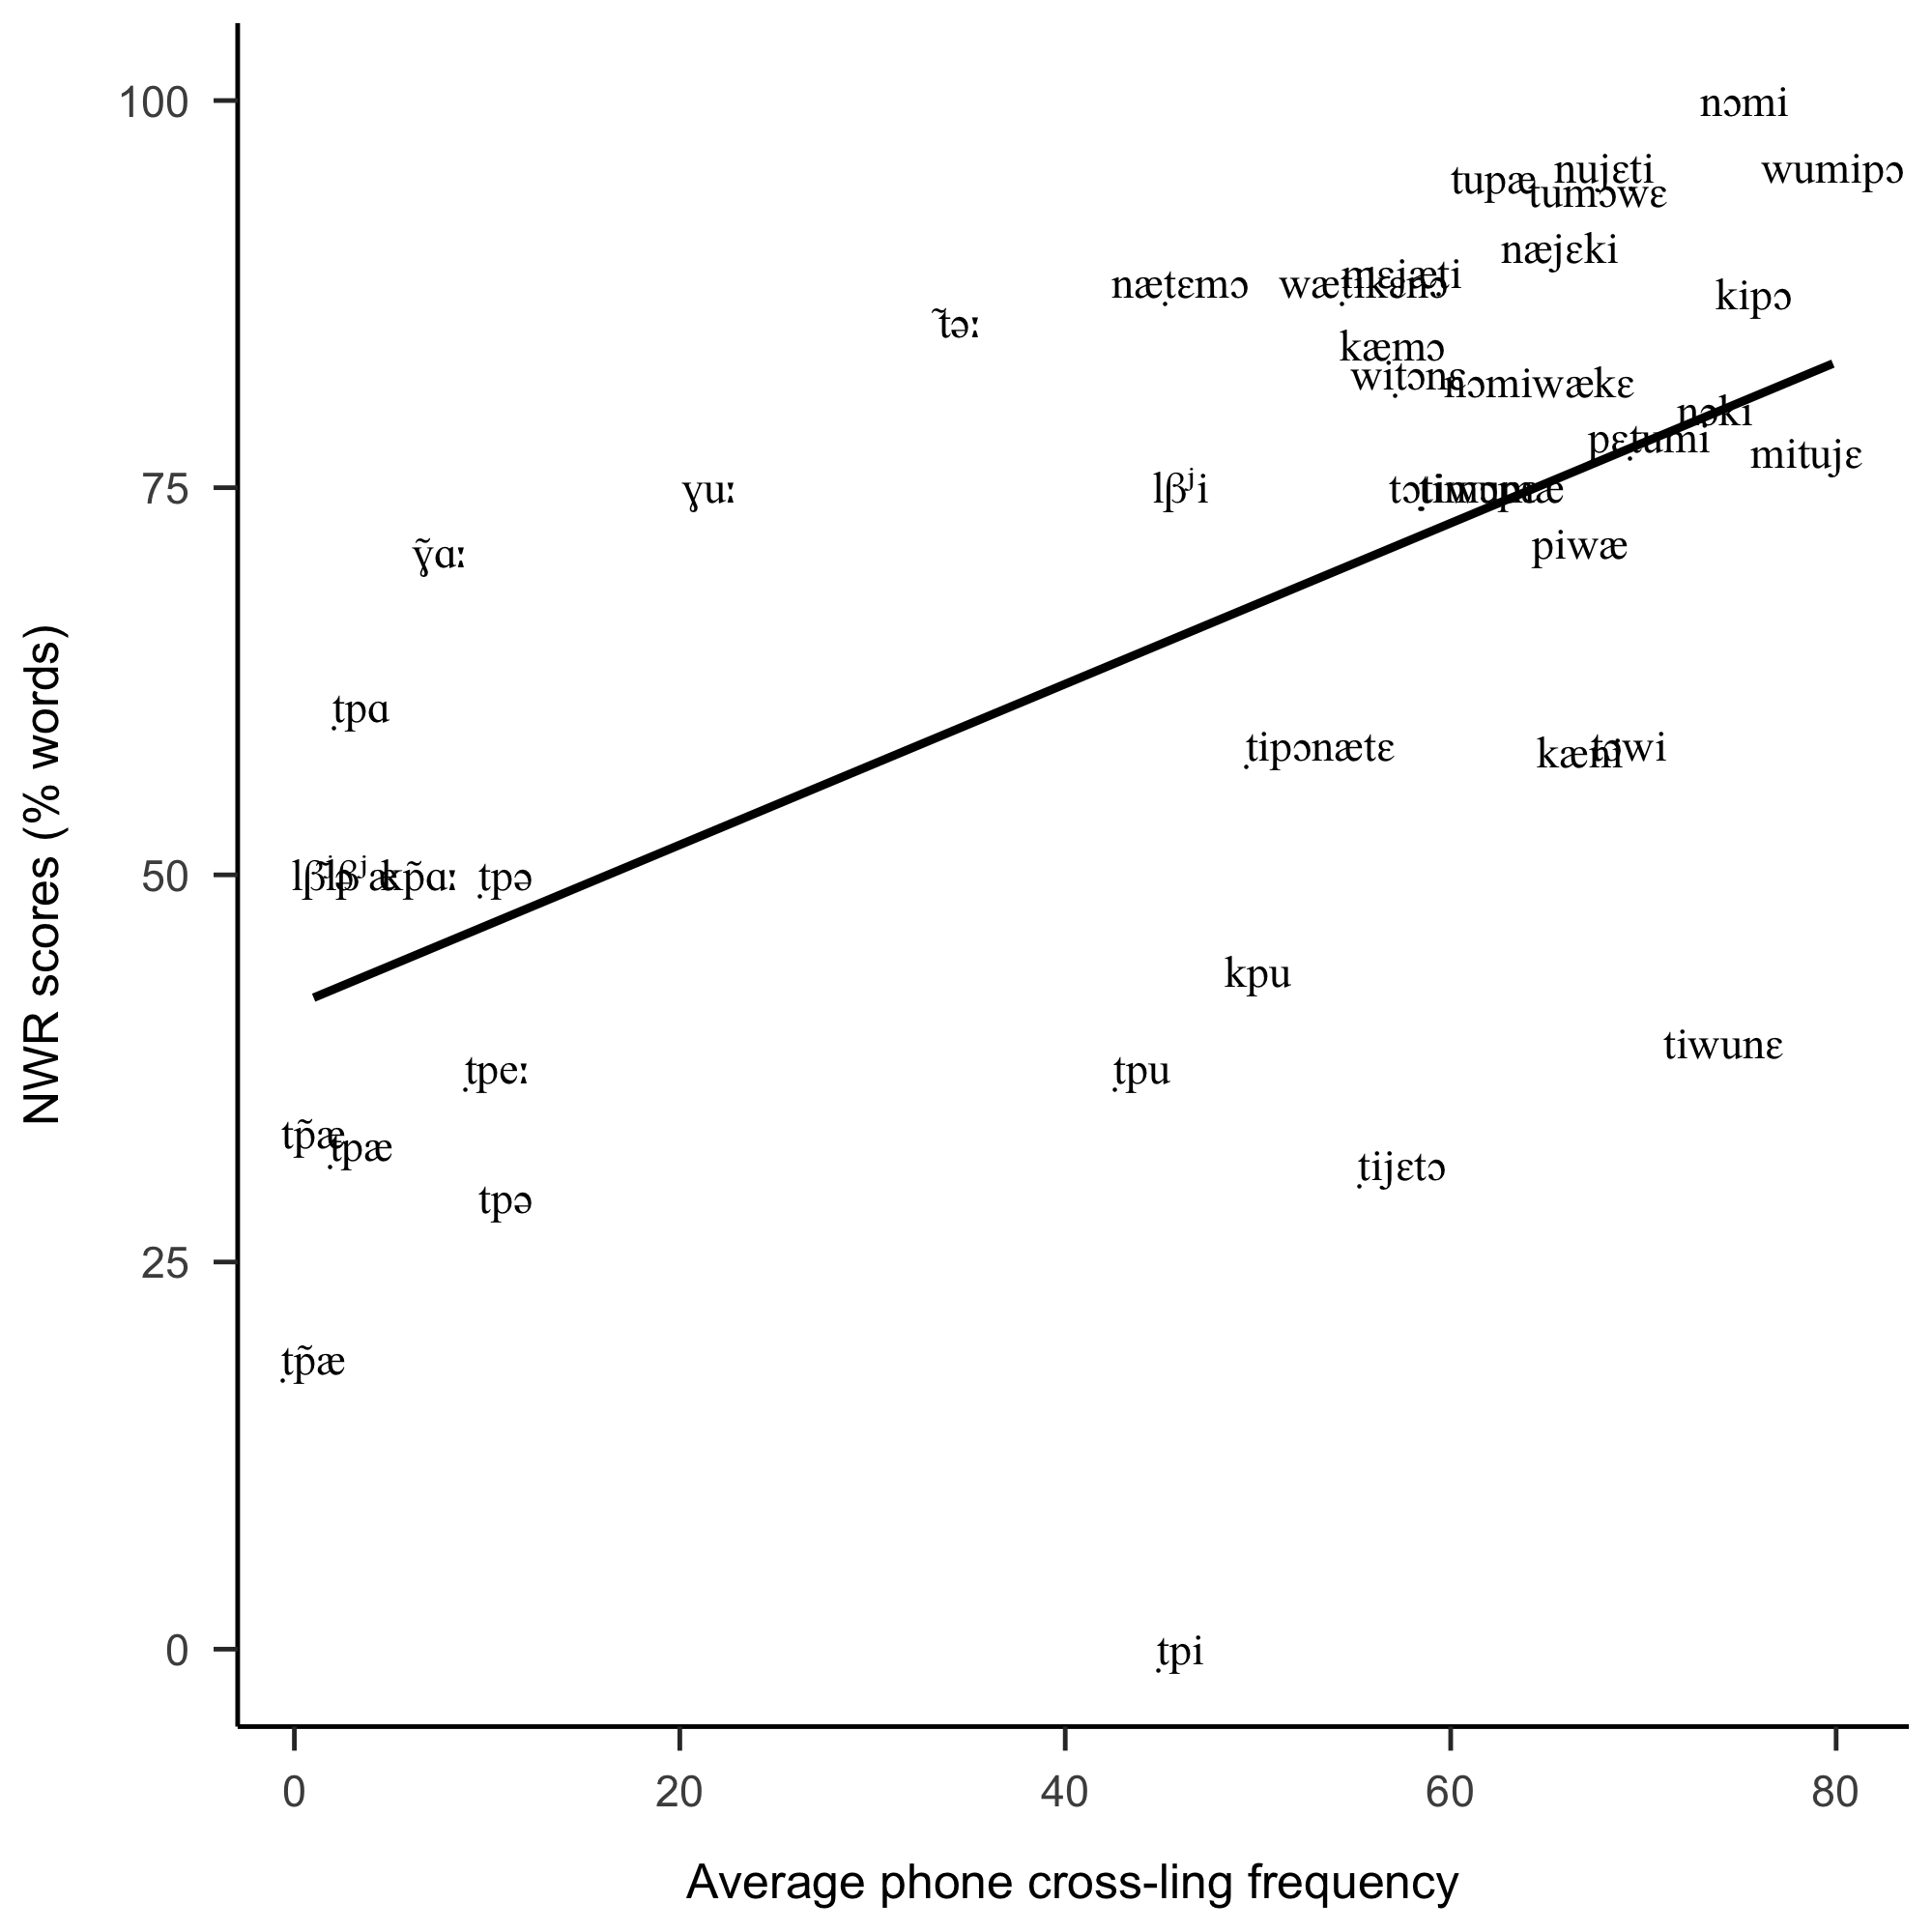
\includegraphics[width=0.65\linewidth]{nwr.by.freq.ITEM} 

}

\caption{NWR scores for individual target words as a function of the average frequency with which each phone is found across languages.}\label{fig:Fig2-xling-freq}
\end{figure}

We next checked whether the association between whole-item NWR scores
and cross-linguistic phone frequence is actually be due to frequency of
the sounds within the language: One can suppose that sounds that occur
more frequently across languages are also more frequent within a
language, and therefore may be easier for children to represent and
repeat. We estimated frequency of the phones present in the stimuli in a
corpus of child-centered recordings (Casillas et al., 2020) by counting
the number of word types in which they occurred, and applied the natural
logarithm.\footnote{We also carried out this analysis using token phone
  frequency, but this measure was not correlated with whole-item NWR
  scores, and therefore the fact that it did not explain away the
  predictive value of cross-linguistic phone frequency was less
  informative than the relationship discussed in the main text, with
  type frequencies.} As before, unattested sounds were not considered
(i.e., they were declared NA so that they do not count for analyses).
Phone frequencies estimated from this corpus were correlated with
cross-linguistic phone frequencies (r(27)=0.52, =0.00). Moreover,
averaging across items and participants, the Pearson correlation between
scaled average corpus phone frequency and whole-item NWR scores was r =
0.46. Therefore, we fit another mixed logistic regression, this time
declaring as fixed effects both scaled cross-linguistic and corpus
frequencies (averaged across all attested phones within each stimulus
item), in addition to age. As before, the model contained random slopes
for both child ID and target. In this model, both cross-linguistic
frequency (ß = 0.82, SE ß = 0.27, p = 0.00) and age (ß = 0.33, SE ß =
0.13, p = 0.01) were significant predictors of whole-item NWR scores,
but corpus frequency (ß = 0.00, SE ß = 0.25, p = 1.00) was not.

\subsubsection{Patterns in NWR
mispronunciations}\label{patterns-in-nwr-mispronunciations}

\textbf{Option 1: just numbers, first attempts only } Next, we
investigated patterns of deletion and substitution. Deletions were
relatively rare, with only 7 vowels deleted, and 3 consonants.

As for substitutions, it was as common for a nasal vowel to be produced
as an oral vowel as vice versa (34 oral target vowels produced as nasal
vowels, 30 nasal target vowels produced as oral vowels). Substitutions
in which the oral nature was preserved but the quality of the vowel was
changed were a great deal more common than changes in quality among
nasal vowels (110 oral vowels produced with a different quality; 13
nasal vowels produced with a different quality). As for consonants,
asymmetries were very marked with more complex consonants (specifically
dptpkpkmknmbghlv) mispronounced as simple ones (specifically
mńlwyvdgptkfhch, 115) than vice versa (2). Simple consonants were
mispronounced as other simple consonants quite frequently (68 simple
consonants mispronounced as other simple ones, compared to 33 complex
ones).

\textbf{Option 2: numbers and proportions, first attempts only} Next, we
investigated patterns of deletion and substitution. Deletions were
relatively rare, with only 7 vowels deleted (about 0.23\% of all vowel
targets), and 3 consonants deleted (about 0.12\% of all consonant
targets).

As for substitutions, it was as common for a nasal vowel to be produced
as an oral vowel as vice versa (34 oral target vowels produced as nasal
vowels or about 0.99\% out of all oral vowel targets, 30 nasal target
vowels produced as oral vowels or about 2.37\% out of all nasal vowel
targets). Substitutions in which the oral nature was preserved but the
quality of the vowel was changed were a great deal more common than
changes in quality among nasal vowels (110 oral vowels produced with a
different quality or about 1.86\% out of all oral vowel targets; 13
nasal vowels produced with a different quality or about 2.06\% out of
all nasal vowel targets). As for consonants, asymmetries were very
marked with more complex consonants (specifically dptpkpkmknmbghlv)
mispronounced as simple ones (specifically mńlwyvdgptkfhch, 115 times or
about 1.96\% out of all complex consonant targets) than vice versa (2
times or about 1.96\% out of all simple consonant targets). Simple
consonants were mispronounced as other simple consonants quite
frequently (68 simple consonants mispronounced as other simple ones or
about 0.38\% out of all simple consonant targets, compared to 33 complex
ones or about 1.02\% out of all complex consonant targets).

\textbf{Option 3: numbers and proportions, ALL attempts} Next, we
investigated patterns of deletion and substitution. Deletions were
relatively rare, with only 12 vowels deleted (about 0.28\% of all vowel
targets), and 6 consonants deleted (about 0.19\% of all consonant
targets).

As for substitutions, it was as common for a nasal vowel to be produced
as an oral vowel as vice versa (52 oral target vowels produced as nasal
vowels or about 1.10\% out of all oral vowel targets, 58 nasal target
vowels produced as oral vowels or about 2.53\% out of all nasal vowel
targets). Substitutions in which the oral nature was preserved but the
quality of the vowel was changed were a great deal more common than
changes in quality among nasal vowels (205 oral vowels produced with a
different quality or about 2.16\% out of all oral vowel targets; 23
nasal vowels produced with a different quality or about 2.36\% out of
all nasal vowel targets). As for consonants, asymmetries were very
marked with more complex consonants (specifically dptpkpkmknmbghlv)
mispronounced as simple ones (specifically mńlwyvdgptkfhch, 250 times or
about 2.43\% out of all complex consonant targets) than vice versa (2
times about 2.43\% out of all simple consonant targets). Simple
consonants were mispronounced as other simple consonants quite
frequently (120 simple consonants mispronounced as other simple ones or
about 0.52\% out of all simple consonant targets, compared to 55 complex
ones or about 0.98\% out of all complex consonant targets).

Finally, we looked into the frequency with which mispronunciations
resulted in real words. Two thirds of them were: 63\%. This is a type of
analysis that is seldom reported, and we could only find one comparison
point: ({\textbf{???}}) found that illiterate adults NWR
mispronunciations resulted in real words in 11.16\% of cases, whereas
literate adults did so in only 1.71\%. The percentage we observe here is
much higher than this, but we do not know whether age, language, or even
test structure explains this difference.

\subsubsection{NWR scores as a function of item
length}\label{nwr-scores-as-a-function-of-item-length}

Next, we inspected whether NWR scores varied as a function of word
length. Results are shown on table XX. This table shows that scores for
monosyllables was much lower than for other lengths. This is likely due
to the fact that the majority of monosyllables included were chosen
because they had sounds that are rare in the world's languages, which
may indicate that they are hard to produce or to perceive.

Setting monosyllables aside, we observe the typical pattern of lower
scores for longer items, although this is particularly salient for the
whole word scoring. This is the most commonly reported type of score,
but it is also the least forgiving. The pattern is less marked when
other two scores are used, which are less sensitive to errors. Averaging
across participants and items, the Pearson correlation between length
(2-4 syllables) and whole-item NWR scores was r(1) = -0.91. In a
generalized binomial mixed model, we included 479 observations, from 40
children producing in any given trial one of 24 potential target words.
The analysis revealed a main effect of age (ß = 0.56, SE ß = 0.14, p =
0); and a significant estimate for the length of the target words in
number of syllables (ß = -0.15, SE ß = 0.33, p = 0.65).

\begin{table}[tbp]
\begin{center}
\begin{threeparttable}
\caption{\label{tab:tablength}NWR measured in whole-word scores, phoneme-based scores, and normalized Levenshtein Distance, separately for the four stimuli lengths.}
\begin{tabular}{lll}
\toprule
Word & \multicolumn{1}{c}{Phoneme} & \multicolumn{1}{c}{NLD}\\
\midrule
47 (22) & 59 (17) & 41 (17)\\
79 (22) & 92 (9) & 8 (9)\\
78 (19) & 93 (7) & 7 (7)\\
74 (32) & 91 (12) & 9 (12)\\
\bottomrule
\end{tabular}
\end{threeparttable}
\end{center}
\end{table}

\subsubsection{Factor structuring individual
variation}\label{factor-structuring-individual-variation}

\begin{figure}
\centering
\includegraphics{manuscript_files/figure-latex/Fig2-scores by age-1.pdf}
\caption{(\#fig:Fig2-scores by age)NWR whole-word scores for individual
participants as a function of age and sex (blue = boys, pink = girls).}
\end{figure}

Our final exploratory analysis assessed whether variation in scores was
structured by factors that vary across individuals. As shown in Figure
2, there was a greater deal of variance in earlier than later ages, with
significantly higher NWR scores for older children (Spearman's rank
correlation, given inequality of variance, rho (6,014.70) = 0.44, p =
0.00). In contrast, there was no clear association between NWR scores,
on the one hand, and sex (t (-0.29) = 27.56, p = 0.77), birth order
(data missing for 15 children, rho = (3,441.90) = -0.18, p = 0.39) or
maternal education (data missing for 0 children, rho = ( 9,594.37) =
0.10, p = 0.54).

\subsection{Discussion}\label{discussion}

\begin{itemize}
\item
  What is the overall repetition scores (whole word, phoneme based,
  distance)?
\item
  How does this change as a function of item complexity (number of
  syllables, sound complexity)?
\end{itemize}

\begin{enumerate}
\def\labelenumi{\arabic{enumi}.}
\item
  Prediction based on previous work: Children have higher scores for
  shorter items
\item
  Prediction for Yélî made before seeing the data: The length
  distribution in Yélî words is more balanced than that in English, and
  thus the score decline for poly- versus mono-syllables may be less
  pronounced than that for English.
\item
  it turns out we were right! the scores for 2-4 syll words decline only
  slightly with length
\item
  Prediction based on previous work: Similarly, we do not know of NWR
  research that manipulates the difficulty of the sounds that are
  included in the items, but word naming and other research suggests
  that children achieve higher scores when producing easy and/or
  typologically common sounds than difficult and/or typologically rare
  sounds {[}CITE{]}. Therefore, we expect higher scores for items with
  common sounds than in those with rare sounds.
\item
  Prediction for Yélî made before seeing the data: The Yélî sound
  inventory is very large and compressed, with many similar sounds that
  are acoustic and articulatory neighbors. Therefore, this may
  constitute a pressure for children to have finer auditory skills (and
  perhaps more precise articulations) than children speaking languages
  with a simpler inventory. As a result, differences between easier and
  harder items may be smaller in this work than in other research.
\item
  it turns out we do see
\end{enumerate}

\begin{itemize}
\tightlist
\item
  How frequent are errors that result in real words? Is that a function
  of item complexity?
\item
  Is individual variation explainable by child age, sex, birth order,
  monolingual status, and/or parental education?
\end{itemize}

\begin{enumerate}
\def\labelenumi{\arabic{enumi}.}
\setcounter{enumi}{2}
\item
  Children's scores increases with child age.
\item
  General prediction: Non-monolingual Yélî children have lower scores
  than monolingual ones when tested on the society-dominant language (we
  did not test any non-dominant language) 
\item
  Local prediction: Anecdotally Yélî children grow up in close-knitted
  communities and thus may receive significant portions of their
  language input from people not in their nuclear family (or at least
  from people other than their mothers, who tend to be the non-native
  speakers). If so, the difference between monolinguals and not
  monolinguals may be smaller than that found in other work . That said,
  one recent study on the same population shows that most child-directed
  input in the first 2 years does come from the mother , so in so far as
  this input has a crucial formational role, then there may still be a
  score difference between these two groups.
\item
  We don't see a difference
\item
  General prediction: previous NWR evidence on this is mixed, but
  general findings on language development suggest that children whose
  mothers are more educated score higher in standardized language tests
  (eg ppvt) than children whose mothers are less educated.
\item
  Prediction made before seeing data: In the Rossel community, formal
  education plays an extremely minor role in ensuring individual's
  success, is not a good index of relative socio-economic status, and
  furthermore there is only a narrow range of variation in maternal
  educational attainment. This may lead to no or only very small
  advantages for children whose mothers are more educated, provided that
  the causal chain between maternal education and child language is via
  SES more broadly. However, if education directly boosts maternal
  verbal skills and the incidence of verbal behavior (as suggested by
  CITE), then we should still see a difference along this factor.
\item
  We did not find this
\item
  General prediction: To our knowledge, there is no previous NWR work on
  this, but other research suggests that first-born children score
  higher in standardized language tests later-born children.
\item
  Prediction before seeing data: One main causal path between birth
  order and language development is via parental input (CITE). Given our
  arguments above for how mothers may not be as important among Rossel
  people than in other places, then the difference in scores between
  first borns and later borns may be small
\item
  we did not find a sig effect, but this is a small effect (eg d=.2 in
  Havron et al)
\end{enumerate}

\newpage

\subsection{Acknowledgments}\label{acknowledgments}

We are grateful to the individuals who participated in the study. The
collection and annotation of these recordings was made possible by
Ndapw:éé Yidika, Taakêmê Ńamono, and Y:aaw:aa Pikuwa; with thanks also
to the PNG National Research Institute, and the Administration of Milne
Bay Province AC acknowledges financial and institutional support from
Agence Nationale de la Recherche (ANR-17-CE28-0007 LangAge,
ANR-16-DATA-0004 ACLEW, ANR-14-CE30-0003 MechELex, ANR-17-EURE-0017) and
the J. S. McDonnell Foundation Understanding Human Cognition Scholar
Award. MC acknowledges financial support from an NWO Veni Innovational
Scheme grant (275-89-033).

\section{References}\label{references}

\setlength{\parindent}{-0.5in} \setlength{\leftskip}{0.5in}

\hypertarget{refs}{}
\hypertarget{ref-is08042009language}{}
Action, C. (2009). Language impairment in a multilingual society:
Linguistic patterns and the road to assessment. \emph{Brussels: COST
Office. Available Online at: Http://Www. Bi-Sli. Org}.

\hypertarget{ref-balladares2016socio}{}
Balladares, J., Marshall, C., \& Griffiths, Y. (2016). Socio-economic
status affects sentence repetition, but not non-word repetition, in
Chilean preschoolers. \emph{First Language}, \emph{36}(3), 338--351.
doi:\href{https://doi.org/10.1177/0142723715626067}{10.1177/0142723715626067}

\hypertarget{ref-bergelsoncasillas2019what}{}
Bergelson, E., Casillas, M., Soderstrom, M., Seidl, A., Warlaumont, A.
S., \& Amatuni, A. (2019). What do North American babies hear? A
large-scale cross-corpus analysis. \emph{Developmental Science},
\emph{22}(1), e12724.
doi:\href{https://doi.org/10.1111/desc.12724}{10.1111/desc.12724}

\hypertarget{ref-Praat}{}
Boersma, P., \& Weenink, D. (2020). Praat: Doing phonetics by computer
(Version 6.1.35). Retrieved from \url{http://www.praat.org/}

\hypertarget{ref-bowey2001nonword}{}
Bowey, J. A. (2001). Nonword repetition and young children's receptive
vocabulary: A longitudinal study. \emph{Applied Psycholinguistics},
\emph{22}(3), 441--469.

\hypertarget{ref-brandeker2015language}{}
Brandeker, M., \& Thordardottir, E. (2015). Language exposure in
bilingual toddlers: Performance on nonword repetition and lexical tasks.
\emph{American Journal of Speech-Language Pathology}, \emph{24}(2),
126--138.

\hypertarget{ref-brown2011cultural}{}
Brown, P. (2011). The cultural organization of attention. In A. Duranti,
E. Ochs, \& and Bambi B Schieffelin (Eds.), \emph{Handbook of Language
Socialization} (pp. 29--55). Malden, MA: Wiley-Blackwell.

\hypertarget{ref-brown2014interactional}{}
Brown, P. (2014). The interactional context of language learning in
Tzeltal. In I. Arnon, M. Casillas, C. Kurumada, \& B. Estigarribia
(Eds.), \emph{Language in interaction: Studies in honor of Eve V. Clark}
(pp. 51--82). Amsterdam, NL: John Benjamins.

\hypertarget{ref-brownIPchildrearing}{}
Brown, P., \& Casillas, M. (in press). Childrearing through social
interaction on Rossel Island, PNG. In A. J. Fentiman \& M. Goody (Eds.),
\emph{Esther Goody revisited: Exploring the legacy of an original
inter-disciplinarian} (pp. XX--XX). New York, NY: Berghahn.

\hypertarget{ref-bunceURcrosscultural}{}
Bunce, J., Soderstrom, M., Bergelson, E., Rosemberg, C., Stein, A.,
Alam, F., \ldots{} Casillas, M. (under review). A cross-cultural
examination of young children's everyday language experiences.

\hypertarget{ref-casillas2020early}{}
Casillas, M., Brown, P., \& Levinson, S. C. (2020). Early language
experience in a papuan community. \emph{Journal of Child Language},
\emph{XX}, XX--XX.

\hypertarget{ref-chiat2007preschool}{}
Chiat, S., \& Roy, P. (2007). The preschool repetition test: An
evaluation of performance in typically developing and clinically
referred children. \emph{Journal of Speech, Language, and Hearing
Research}, \emph{50}(2), 429--443.

\hypertarget{ref-cristia2020infant}{}
Cristia, A., Farabolini, G., Scaff, C., Havron, N., \& Stieglitz, J.
(2020). Infant-directed input and literacy effects on phonological
processing: Non-word repetition scores among the tsimane'.
\emph{Preprint}.

\hypertarget{ref-estes2007differences}{}
Estes, K. G., Evans, J. L., \& Else-Quest, N. M. (2007). Differences in
the nonword repetition performance of children with and without specific
language impairment: A meta-analysis. \emph{Journal of Speech, Language,
and Hearing Research}, \emph{50}(1), 177--195.

\hypertarget{ref-farmani2018normalization}{}
Farmani, H., Sayyahi, F., Soleymani, Z., Labbaf, F. Z., Talebi, E., \&
Shourvazi, Z. (2018). Normalization of the non-word repetition test in
farsi-speaking children. \emph{Journal of Modern Rehabilitation},
\emph{12}(4), 217--224.

\hypertarget{ref-foley1986papuan}{}
Foley, W. A. (1986). \emph{The papuan languages of new guinea}.
Cambridge, UK: Cambridge University Press.

\hypertarget{ref-gallagher2014identity}{}
Gallagher, G. (2014). An identity bias in phonotactics: Evidence from
Cochabamba Quechua. \emph{Laboratory Phonology}, \emph{5}(3), 337--378.
doi:\href{https://doi.org/10.1515/lp-2014-0012}{10.1515/lp-2014-0012}

\hypertarget{ref-gallon2007non}{}
Gallon, N., Harris, J., \& Van der Lely, H. (2007). Non-word repetition:
An investigation of phonological complexity in children with grammatical
sli. \emph{Clinical Linguistics \& Phonetics}, \emph{21}(6), 435--455.

\hypertarget{ref-havron2019effect}{}
Havron, N., Ramus, F., Heude, B., Forhan, A., Cristia, A., Peyre, H., \&
Group, E. M.-C. C. S. (2019). The effect of older siblings on language
development as a function of age difference and sex. \emph{Psychological
Science}, \emph{30}(9), 1333--1343.

\hypertarget{ref-hazan2000development}{}
Hazan, V., \& Barrett, S. (2000). The development of phonemic
categorization in children aged 6--12. \emph{Journal of Phonetics},
\emph{28}(4), 377--396.

\hypertarget{ref-jabere2018xperiment}{}
Jaber-Awida, A. (2018). Experiment in non word repetition by monolingual
Arabic preschoolers. \emph{Athens Journal of Philology}, \emph{5}(4),
317--334.
doi:\href{https://doi.org/10.30958/ajp.5-4-4}{10.30958/ajp.5-4-4}

\hypertarget{ref-kalnak2014nonword}{}
Kalnak, N., Peyrard-Janvid, M., Forssberg, H., \& Sahlén, B. (2014).
Nonword repetition--a clinical marker for specific language impairment
in swedish associated with parents' language-related problems.
\emph{PloS One}, \emph{9}(2), e89544.

\hypertarget{ref-ladefoged1996sounds}{}
Ladefoged, P., \& Maddieson, I. (1996). \emph{The sounds of the world's
languages} (Vol. 1012). Blackwell Oxford.

\hypertarget{ref-levinsonYDgrammar}{}
Levinson, S. C. (accepted). \emph{A grammar of yélî dnye, the papuan
language of rossel island}. Berlin, Boston: De Gruyter Mouton.

\hypertarget{ref-liszkowski2012prelinguistic}{}
Liszkowski, U., Brown, P., Callaghan, T., Takada, A., \& de Vos, C.
(2012). A prelinguistic gestural universal of human communication.
\emph{Cognitive Science}, \emph{36}(4), 698--713.
doi:\href{https://doi.org/10.1111/j.1551-6709.2011.01228.x}{10.1111/j.1551-6709.2011.01228.x}

\hypertarget{ref-maddieson2005correlating}{}
Maddieson, I. (2005). Correlating phonological complexity: Data and
validation. \emph{UC Berkeley PhonLab Annual Report}, \emph{1}(1).

\hypertarget{ref-maddiesonIPphoneticsYD}{}
Maddieson, I., \& Levinson, S. C. (in preparation). \emph{The phonetics
of yélî dnye, the language of rossel island}.

\hypertarget{ref-meir2017independent}{}
Meir, N., \& Armon-Lotem, S. (2017). Independent and combined effects of
socioeconomic status (ses) and bilingualism on children's vocabulary and
verbal short-term memory. \emph{Frontiers in Psychology}, \emph{8},
1442.

\hypertarget{ref-meir2016disentangling}{}
Meir, N., Walters, J., \& Armon-Lotem, S. (2016). Disentangling sli and
bilingualism using sentence repetition tasks: The impact of l1 and l2
properties. \emph{International Journal of Bilingualism}, \emph{20}(4),
421--452.

\hypertarget{ref-phoible}{}
Moran, S., \& McCloy, D. (Eds.). (2019). \emph{PHOIBLE 2.0}. Jena: Max
Planck Institute for the Science of Human History. Retrieved from
\url{https://phoible.org/}

\hypertarget{ref-peuteIPconsonants}{}
Peute, A. A. K., Fikkert, P., \& Casillas, M. (In preparation). Early
consonant production in Yélî Dnye and Tseltal.

\hypertarget{ref-piazzalunga2019articulatory}{}
Piazzalunga, S., Previtali, L., Pozzoli, R., Scarponi, L., \& Schindler,
A. (2019). An articulatory-based disyllabic and trisyllabic non-word
repetition test: Reliability and validity in italian 3-to 7-year-old
children. \emph{Clinical Linguistics \& Phonetics}, \emph{33}(5),
437--456.

\hypertarget{ref-torrington2015non}{}
Torrington Eaton, C., Newman, R. S., Ratner, N. B., \& Rowe, M. L.
(2015). Non-word repetition in 2-year-olds: Replication of an adapted
paradigm and a useful methodological extension. \emph{Clinical
Linguistics \& Phonetics}, \emph{29}(7), 523--535.

\hypertarget{ref-vance2005speech}{}
Vance, M., Stackhouse, J., \& Wells, B. (2005). Speech-production skills
in children aged 3--7 years. \emph{International Journal of Language \&
Communication Disorders}, \emph{40}(1), 29--48.

\hypertarget{ref-wilsenach2013phonological}{}
Wilsenach, C. (2013). Phonological skills as predictor of reading
success: An investigation of emergent bilingual Northern Sotho/English
learners. \emph{Per Linguam: a Journal of Language Learning= Per
Linguam: Tydskrif vir Taalaanleer}, \emph{29}(2), 17--32.
doi:\href{https://doi.org/10.5785/29-2-554}{10.5785/29-2-554}

\hypertarget{ref-is08042009language}{}
Action, C. (2009). Language impairment in a multilingual society:
Linguistic patterns and the road to assessment. \emph{Brussels: COST
Office. Available Online at: Http://Www. Bi-Sli. Org}.

\hypertarget{ref-balladares2016socio}{}
Balladares, J., Marshall, C., \& Griffiths, Y. (2016). Socio-economic
status affects sentence repetition, but not non-word repetition, in
Chilean preschoolers. \emph{First Language}, \emph{36}(3), 338--351.
doi:\href{https://doi.org/10.1177/0142723715626067}{10.1177/0142723715626067}

\hypertarget{ref-bergelsoncasillas2019what}{}
Bergelson, E., Casillas, M., Soderstrom, M., Seidl, A., Warlaumont, A.
S., \& Amatuni, A. (2019). What do North American babies hear? A
large-scale cross-corpus analysis. \emph{Developmental Science},
\emph{22}(1), e12724.
doi:\href{https://doi.org/10.1111/desc.12724}{10.1111/desc.12724}

\hypertarget{ref-Praat}{}
Boersma, P., \& Weenink, D. (2020). Praat: Doing phonetics by computer
(Version 6.1.35). Retrieved from \url{http://www.praat.org/}

\hypertarget{ref-bowey2001nonword}{}
Bowey, J. A. (2001). Nonword repetition and young children's receptive
vocabulary: A longitudinal study. \emph{Applied Psycholinguistics},
\emph{22}(3), 441--469.

\hypertarget{ref-brandeker2015language}{}
Brandeker, M., \& Thordardottir, E. (2015). Language exposure in
bilingual toddlers: Performance on nonword repetition and lexical tasks.
\emph{American Journal of Speech-Language Pathology}, \emph{24}(2),
126--138.

\hypertarget{ref-brown2011cultural}{}
Brown, P. (2011). The cultural organization of attention. In A. Duranti,
E. Ochs, \& and Bambi B Schieffelin (Eds.), \emph{Handbook of Language
Socialization} (pp. 29--55). Malden, MA: Wiley-Blackwell.

\hypertarget{ref-brown2014interactional}{}
Brown, P. (2014). The interactional context of language learning in
Tzeltal. In I. Arnon, M. Casillas, C. Kurumada, \& B. Estigarribia
(Eds.), \emph{Language in interaction: Studies in honor of Eve V. Clark}
(pp. 51--82). Amsterdam, NL: John Benjamins.

\hypertarget{ref-brownIPchildrearing}{}
Brown, P., \& Casillas, M. (in press). Childrearing through social
interaction on Rossel Island, PNG. In A. J. Fentiman \& M. Goody (Eds.),
\emph{Esther Goody revisited: Exploring the legacy of an original
inter-disciplinarian} (pp. XX--XX). New York, NY: Berghahn.

\hypertarget{ref-bunceURcrosscultural}{}
Bunce, J., Soderstrom, M., Bergelson, E., Rosemberg, C., Stein, A.,
Alam, F., \ldots{} Casillas, M. (under review). A cross-cultural
examination of young children's everyday language experiences.

\hypertarget{ref-casillas2020early}{}
Casillas, M., Brown, P., \& Levinson, S. C. (2020). Early language
experience in a papuan community. \emph{Journal of Child Language},
\emph{XX}, XX--XX.

\hypertarget{ref-chiat2007preschool}{}
Chiat, S., \& Roy, P. (2007). The preschool repetition test: An
evaluation of performance in typically developing and clinically
referred children. \emph{Journal of Speech, Language, and Hearing
Research}, \emph{50}(2), 429--443.

\hypertarget{ref-cristia2020infant}{}
Cristia, A., Farabolini, G., Scaff, C., Havron, N., \& Stieglitz, J.
(2020). Infant-directed input and literacy effects on phonological
processing: Non-word repetition scores among the tsimane'.
\emph{Preprint}.

\hypertarget{ref-estes2007differences}{}
Estes, K. G., Evans, J. L., \& Else-Quest, N. M. (2007). Differences in
the nonword repetition performance of children with and without specific
language impairment: A meta-analysis. \emph{Journal of Speech, Language,
and Hearing Research}, \emph{50}(1), 177--195.

\hypertarget{ref-farmani2018normalization}{}
Farmani, H., Sayyahi, F., Soleymani, Z., Labbaf, F. Z., Talebi, E., \&
Shourvazi, Z. (2018). Normalization of the non-word repetition test in
farsi-speaking children. \emph{Journal of Modern Rehabilitation},
\emph{12}(4), 217--224.

\hypertarget{ref-foley1986papuan}{}
Foley, W. A. (1986). \emph{The papuan languages of new guinea}.
Cambridge, UK: Cambridge University Press.

\hypertarget{ref-gallagher2014identity}{}
Gallagher, G. (2014). An identity bias in phonotactics: Evidence from
Cochabamba Quechua. \emph{Laboratory Phonology}, \emph{5}(3), 337--378.
doi:\href{https://doi.org/10.1515/lp-2014-0012}{10.1515/lp-2014-0012}

\hypertarget{ref-gallon2007non}{}
Gallon, N., Harris, J., \& Van der Lely, H. (2007). Non-word repetition:
An investigation of phonological complexity in children with grammatical
sli. \emph{Clinical Linguistics \& Phonetics}, \emph{21}(6), 435--455.

\hypertarget{ref-havron2019effect}{}
Havron, N., Ramus, F., Heude, B., Forhan, A., Cristia, A., Peyre, H., \&
Group, E. M.-C. C. S. (2019). The effect of older siblings on language
development as a function of age difference and sex. \emph{Psychological
Science}, \emph{30}(9), 1333--1343.

\hypertarget{ref-hazan2000development}{}
Hazan, V., \& Barrett, S. (2000). The development of phonemic
categorization in children aged 6--12. \emph{Journal of Phonetics},
\emph{28}(4), 377--396.

\hypertarget{ref-jabere2018xperiment}{}
Jaber-Awida, A. (2018). Experiment in non word repetition by monolingual
Arabic preschoolers. \emph{Athens Journal of Philology}, \emph{5}(4),
317--334.
doi:\href{https://doi.org/10.30958/ajp.5-4-4}{10.30958/ajp.5-4-4}

\hypertarget{ref-kalnak2014nonword}{}
Kalnak, N., Peyrard-Janvid, M., Forssberg, H., \& Sahlén, B. (2014).
Nonword repetition--a clinical marker for specific language impairment
in swedish associated with parents' language-related problems.
\emph{PloS One}, \emph{9}(2), e89544.

\hypertarget{ref-ladefoged1996sounds}{}
Ladefoged, P., \& Maddieson, I. (1996). \emph{The sounds of the world's
languages} (Vol. 1012). Blackwell Oxford.

\hypertarget{ref-levinsonYDgrammar}{}
Levinson, S. C. (accepted). \emph{A grammar of yélî dnye, the papuan
language of rossel island}. Berlin, Boston: De Gruyter Mouton.

\hypertarget{ref-liszkowski2012prelinguistic}{}
Liszkowski, U., Brown, P., Callaghan, T., Takada, A., \& de Vos, C.
(2012). A prelinguistic gestural universal of human communication.
\emph{Cognitive Science}, \emph{36}(4), 698--713.
doi:\href{https://doi.org/10.1111/j.1551-6709.2011.01228.x}{10.1111/j.1551-6709.2011.01228.x}

\hypertarget{ref-maddieson2005correlating}{}
Maddieson, I. (2005). Correlating phonological complexity: Data and
validation. \emph{UC Berkeley PhonLab Annual Report}, \emph{1}(1).

\hypertarget{ref-maddiesonIPphoneticsYD}{}
Maddieson, I., \& Levinson, S. C. (in preparation). \emph{The phonetics
of yélî dnye, the language of rossel island}.

\hypertarget{ref-meir2017independent}{}
Meir, N., \& Armon-Lotem, S. (2017). Independent and combined effects of
socioeconomic status (ses) and bilingualism on children's vocabulary and
verbal short-term memory. \emph{Frontiers in Psychology}, \emph{8},
1442.

\hypertarget{ref-meir2016disentangling}{}
Meir, N., Walters, J., \& Armon-Lotem, S. (2016). Disentangling sli and
bilingualism using sentence repetition tasks: The impact of l1 and l2
properties. \emph{International Journal of Bilingualism}, \emph{20}(4),
421--452.

\hypertarget{ref-phoible}{}
Moran, S., \& McCloy, D. (Eds.). (2019). \emph{PHOIBLE 2.0}. Jena: Max
Planck Institute for the Science of Human History. Retrieved from
\url{https://phoible.org/}

\hypertarget{ref-peuteIPconsonants}{}
Peute, A. A. K., Fikkert, P., \& Casillas, M. (In preparation). Early
consonant production in Yélî Dnye and Tseltal.

\hypertarget{ref-piazzalunga2019articulatory}{}
Piazzalunga, S., Previtali, L., Pozzoli, R., Scarponi, L., \& Schindler,
A. (2019). An articulatory-based disyllabic and trisyllabic non-word
repetition test: Reliability and validity in italian 3-to 7-year-old
children. \emph{Clinical Linguistics \& Phonetics}, \emph{33}(5),
437--456.

\hypertarget{ref-torrington2015non}{}
Torrington Eaton, C., Newman, R. S., Ratner, N. B., \& Rowe, M. L.
(2015). Non-word repetition in 2-year-olds: Replication of an adapted
paradigm and a useful methodological extension. \emph{Clinical
Linguistics \& Phonetics}, \emph{29}(7), 523--535.

\hypertarget{ref-vance2005speech}{}
Vance, M., Stackhouse, J., \& Wells, B. (2005). Speech-production skills
in children aged 3--7 years. \emph{International Journal of Language \&
Communication Disorders}, \emph{40}(1), 29--48.

\hypertarget{ref-wilsenach2013phonological}{}
Wilsenach, C. (2013). Phonological skills as predictor of reading
success: An investigation of emergent bilingual Northern Sotho/English
learners. \emph{Per Linguam: a Journal of Language Learning= Per
Linguam: Tydskrif vir Taalaanleer}, \emph{29}(2), 17--32.
doi:\href{https://doi.org/10.5785/29-2-554}{10.5785/29-2-554}

\end{document}
